% Corps du contrôle - Fractions décimales et nombres décimaux

% === Barème avec nouvelle fonction ===
\bareme{
	\exbadge{1}{6} \quad
	\exbadge{2}{5} \quad
	\exbadge{3}{4} \quad
	\exbadge{4}{5}
}

% === Consignes ===
\begin{consignebox}
	\faIcon{info-circle} \textbf{CONSIGNES IMPORTANTES}
	\begin{itemize}[leftmargin=*,noitemsep,topsep=5pt]
		\item[\faIcon{check}] Répondez directement sur le sujet
		\item[\faIcon{check}] Justifiez vos réponses quand c'est demandé
		\item[\faIcon{pencil-alt}] Écrivez lisiblement
		\item[\faIcon{calculator}] Calculatrice autorisée
	\end{itemize}
\end{consignebox}

\smallspace

% ============================================
% EXERCICE 1 : Fractions décimales et représentations (6 points)
% ============================================
\ExTemplate{1}{Fractions décimales et représentations}{6}{book}{
\textbf{1.} Parmi les fractions suivantes, entoure uniquement les fractions décimales : \points{1,5}

\smallspace

$$\dfrac{7}{10} \qquad ; \qquad \dfrac{2}{3} \qquad ; \qquad \dfrac{45}{100} \qquad ; \qquad \dfrac{5}{7} \qquad ; \qquad \dfrac{123}{1~000}$$

\onlycorrige{
\textcolor{red}{Réponse : $\dfrac{7}{10}$, $\dfrac{45}{100}$ et $\dfrac{123}{1~000}$ sont des fractions décimales car leurs dénominateurs sont 10, 100 ou 1~000.}
}

\exspace

\textbf{2.} Représentation visuelle : \points{2}

\smallspace

Colorie le grand carré ci-dessous pour représenter la fraction $\dfrac{37}{100}$ :

\begin{center}
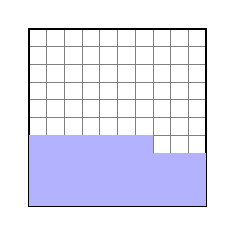
\begin{tikzpicture}[scale=0.45]
	% Grille 10x10
	\draw[step=0.5,gray,very thin] (0,0) grid (5,5);
	\draw[thick] (0,0) rectangle (5,5);

	\onlycorrige{
		% Colorier 37 cases (3 lignes complètes + 7 cases)
		\fill[blue!30] (0,0) rectangle (5,1.5);
		\fill[blue!30] (0,1.5) rectangle (3.5,2);
	}
\end{tikzpicture}
\end{center}

\exspace

\textbf{3.} Complète les phrases suivantes : \points{1,5}

\smallspace

\begin{itemize}[label=$\bullet$,leftmargin=*,noitemsep]
	\item $\dfrac{7}{10}$ se lit : \solution[4cm]{sept dixièmes}
	\item $\dfrac{23}{100}$ se lit : \solution[5cm]{vingt-trois centièmes}
	\item $\dfrac{145}{1~000}$ se lit : \solution[6cm]{cent quarante-cinq millièmes}
\end{itemize}

\exspace

\textbf{4.} Pour le nombre décimal $37{,}84$ : \points{1}

\smallspace

\begin{itemize}[label=$\bullet$,leftmargin=*,noitemsep]
	\item Le chiffre des dixièmes est : \solution[1.5cm]{8}
	\item Le chiffre des millièmes est : \solution[1.5cm]{0}
\end{itemize}
}

\smallspace

% ============================================
% EXERCICE 2 : Différentes écritures d'un nombre décimal (5 points)
% ============================================
\begin{exercisebox}{\faIcon{pen} Exercice 2 : Différentes écritures d'un nombre décimal \points{5}}

	\textbf{1.} Écris les nombres suivants en écriture décimale : \points{2}

	\smallspace

	\begin{itemize}[label=$\bullet$,leftmargin=*,noitemsep]
		\item $\dfrac{34}{10} = $ \solution[2cm]{3,4}
		\item $\dfrac{567}{100} = $ \solution[2cm]{5,67}
		\item $7 + \dfrac{38}{100} = $ \solution[2cm]{7,38}
		\item $\dfrac{2~850}{1~000} = $ \solution[2cm]{2,85}
	\end{itemize}

	\exspace

	\textbf{2.} Écris le nombre $14{,}56$ sous les formes suivantes : \points{2}

	\smallspace

	\begin{itemize}[label=$\bullet$,leftmargin=*,noitemsep]
		\item Fraction décimale : \solution[3.5cm]{$\dfrac{1~456}{100}$}
		\item Partie entière + fraction décimale inférieure à 1 : \solution[4.5cm]{$14 + \dfrac{56}{100}$}
		\item Décomposition additive avec fractions décimales : \solution[7cm]{$10 + 4 + \dfrac{5}{10} + \dfrac{6}{100}$}
	\end{itemize}

	\exspace

	\textbf{3.} Complète : \points{1}

	\smallspace
	
	$8 + \dfrac{61}{100} = $ \solution[3cm]{8,61} \qquad $13{,}402 = $ \solution[1.5cm]{13} $+$ \solution[3cm]{$\dfrac{402}{1~000}$}


\end{exercisebox}

\smallspace

% ============================================
% EXERCICE 3 : Comparer et ranger (4 points)
% ============================================
\begin{exercisebox}{\faIcon{balance-scale} Exercice 3 : Comparer et ranger \points{4}}

	\textbf{1.} Complète avec le symbole $<$, $>$ ou $=$ : \points{2}

	\smallspace

	\setlength{\columnsep}{0.8cm}
	\begin{multicols}{2}
		\begin{enumerate}[itemsep=0.3em, topsep=0.2em, leftmargin=*, label=\alph*)]
			\item $5{,}7 \quad \solution[1cm]{=} \quad 5{,}70$
			\item $12{,}34 \quad \solution[1cm]{<} \quad 12{,}4$
			\item $8{,}099 \quad \solution[1cm]{<} \quad 8{,}1$
			\item $23{,}5 \quad \solution[1cm]{>} \quad 23{,}499$
		\end{enumerate}
	\end{multicols}

	\exspace

	\textbf{2.} Range les nombres suivants dans l'ordre croissant : \points{2}

	\smallspace

	$$7{,}2 \quad ; \quad 7{,}02 \quad ; \quad 7{,}201 \quad ; \quad 7{,}21 \quad ; \quad 6{,}999$$

	\smallspace

	\solution[12cm]{$6{,}999 < 7{,}02 < 7{,}2 < 7{,}201 < 7{,}21$}

\end{exercisebox}

\clearpage

% ============================================
% EXERCICE 4 : Encadrer, placer et problèmes (5 points)
% ============================================
\begin{exercisebox}{\faIcon{ruler-combined} Exercice 4 : Encadrer, placer et problèmes \points{5}}

	\textbf{1.} Encadre le nombre $5{,}738$ respectivement à l'unité, au dixième et au centième : \points{1,5}

	\smallspace

	\begin{multicols}{3}
	\begin{itemize}[label=$\bullet$,leftmargin=*,noitemsep]
		\item \solution[1cm]{5} $< 5{,}738 <$ \solution[1cm]{6}

		\item \solution[1.5cm]{5,7} $< 5{,}738 <$ \solution[1.5cm]{5,8}

		\item \solution[1cm]{5,73} $< 5{,}738 <$ \solution[1.5cm]{5,74}
		
	\end{itemize}
	\end{multicols}

	\exspace

	\textbf{2.} Sur la droite graduée ci-dessous, place les points suivants : \points{1,5}

	\smallspace

	\begin{center}
		\begin{tikzpicture}[scale=1.3]
			\draw[thick, ->] (0,0) -- (11,0);
			\foreach \x in {0,10} {
				\draw (\x,-0.2) -- (\x,0.2);
				\node[below] at (\x,-0.4) {\ifnum\x=0 2\else 3\fi};
			}
			\foreach \x in {1,...,9} {\draw (\x,-0.1) -- (\x,0.1);}

			% Corrigé
			\onlycorrige{
				\fill[blue] (4,0) circle (0.08); \node[above] at (4,0.3) {$A$};
				\fill[red] (7,0) circle (0.08); \node[above] at (7,0.3) {$B$};
				\fill[green!60!black] (1.5,0) circle (0.08); \node[above] at (1.5,0.3) {$C$};
			}
		\end{tikzpicture}
	\end{center}
    
    \begin{multicols}{3}
	\begin{itemize}[label=$\bullet$,leftmargin=*,noitemsep]
		\item Le point $A$ d'abscisse $2{,}4$
		\item Le point $B$ d'abscisse $\dfrac{27}{10}$
		\item Le point $C$ d'abscisse $2{,}15$
	\end{itemize}
	\end{multicols}

	\exspace

	\textbf{3.} Problème : \points{2}

	\smallspace

	Au marché, Marie achète :
	\begin{multicols}{3}
	\begin{itemize}[label=$\bullet$,leftmargin=*,noitemsep]
		\item $\dfrac{75}{100}$ kg de pommes
		\item $1 + \dfrac{2}{10}$ kg de carottes
		\item $\dfrac{450}{1~000}$ kg de fraises
	\end{itemize}
	\end{multicols}

	\smallspace

	\textbf{a)} Écris chaque masse en écriture décimale (en kg) : \points{1}

	\smallspace

	\begin{itemize}[label=$\bullet$,leftmargin=*,noitemsep]
		\item Pommes : \solution[2.5cm]{0,75 kg}
		\item Carottes : \solution[2.5cm]{1,2 kg}
		\item Fraises : \solution[2.5cm]{0,45 kg}
	\end{itemize}

	\smallspace

	\textbf{b)} Quelle est la masse totale des courses de Marie (en kg) ? \points{1}

	\anslines{2}{
		Masse totale = $0{,}75 + 1{,}2 + 0{,}45 = 2{,}4$ kg

		\textbf{Marie a acheté 2,4 kg de courses.}
	}

\end{exercisebox}

% Auto-évaluation
\AutoEval
